\section{Experiments and Evaluation}

\subsection{Datasets}

\subsubsection{BioASQ}
train + evaluate; Pubmed-abstract -> Mesh terms; multiclass prediction; ca. 10k classes; use only structured abstracts -> ca. 4m docs
\todo{AB: distribution of text lengths?}

\subsubsection{DBpedia-NIF}
pre-train (+ evaluate); two Wikipedia articles -> relatedness score; similarity prediction; ca. 5m docs
\todo{AB: distribution of text lengths?}

\subsection{Training and Hyperparameters}
batched gradient descent; max entropy loss; adam optimizer; gradient clipping; dropout; \\
train word embeddings for words not in initial (glove + biomedical) embeddings \\
for relatedness prediction: negative sampling 

\subsection{Results}
total (no pre-training; min 170 occurrences per word type/MeSH tag!; F1-scores): \\
tf-idf: 0.64  > RecNN: 0.63 > flat(sum): 0.60 > RNN: 0.50 \\
different results for different text sizes? -> train \& evaluate on text-size-buckets

\if false
===OLD SRP CONTENT===

We conduct several experiments to evaluate the influence of order awareness and availability of dependency type information to the similarity prediction performance. We test all combinations of the boolean parameters \texttt{dependency available} and \texttt{order aware} and the TF-IDF baseline. In the following, we describe the dataset and the hyperparameter setting. Finally, we present the results including a comparative analysis of errors.

\subsection{Dataset}
We use the SICK corpus\footnote{\url{http://alt.qcri.org/semeval2014/task1/index.php?id=data-and-tools}} \autocite{marelli_sick_2014} for model training and evaluation. The corpus consists of about approximately 10.000 pairs of English sentences based on the 8K ImageFlickr data set\footnote{\url{http://nlp.cs.illinois.edu/
HockenmaierGroup/data.html}} \autocite{hodosh_framing_2013} and the SemEval 2012 STS MSR-Video Description data set\footnote{\url{https://www.cs.york.ac.uk/semeval-2012/task6/index.php\%3Fid=data.html}} \autocite{agirre_semeval-2012_2012} that contain sentences describing the same picture or video. These sentences were linguistically normalized; i.e. Named Entities and complex verb constructions are replaced and subordinates are turned into coordinates. Pairs were manually %expanded to generate candidate pairs that were 
labeled by 10 annotators with one to five point relatedness ratings that are averaged to produce a relatedness score. We rescaled the scores into the interval $[0.0, 1.0]$ to let them fit into our definition of a similarity measure. Table~\ref{tab:sick_examples} shows some examples of the dataset. The mean of the score for both train and test set is approximately $0.63$. The sentences contain $2408$ different token types and have an average length of $9.6$ words.  

We chose the SICK corpus because it was used in the SemEval 2014 task 1\footnote{\url{http://alt.qcri.org/semeval2014/task1/}}, thus it is widely studied and various reference systems exist. Furthermore, as stated by \textcite{marelli_semeval-2014_2014}, this corpus was created to evaluate semantical aware composition without relying on too many external tools and resources (e.g., named-entity recognizers, gazetteers, ontologies).
%mean score: 0.63 * 4.0 + 1.0 = 3.53

\begin{table*}[!htb]
\centering
  \begin{tabular}{p{0.4\textwidth}|p{0.4\textwidth}|c}
    sentence A & sentence B & score \\ \hline \hline
    A man in a shirt dyed purple is looking at a man in a black shirt who is doing a funny face & A man in a shirt dyed purple is looking at a man in a black shirt who is doing a face which looks funny & 1.0 \\ \hline
    A group of kids is playing in a yard and an old man is standing in the background & A group of boys in a yard is playing and a man is standing in the background & 0.875 \\ \hline
    A brown dog is attacking another animal in front of the man in pants & Two dogs are wrestling and hugging & 0.55 \\ \hline
    A woman is chopping an onion & A woman is washing her feet & 0.0
  \end{tabular}
  \caption{Example sentence pairs from SICK corpus with rescaled relatedness score ranging from $0.0$ (not related) to $1.0$ (maximal related).}
\label{tab:sick_examples}
\end{table*}

%\subsubsection{SICK}

%\subsubsection{PPDB}
%Our pre-training dataset is based on the phrasal part of the PPDB 2.0 dataset \autocite{pavlick_ppdb_2015}. We use a subset of 100,000 paraphrases and add an equal amount of negative samples by replacing for each pair the second paraphrase entry with a random phrase sampled uniformly\footnote{We also tried to sample according to the Jaccard similarity distribution of the original pairs, but this decreased the performance.} from all existing second pair entries. A similarity score of 1.0 is assigned to the original paraphrase pairs, the negative samples are scored with 0.0.

\subsection{Training and Hyperparameters}
We train the model in batches of 100 examples. The ADAM optimizer is initialized with a learning rate of 0.003. We apply gradient clipping by global norm as specified in \textcite{pascanu_difficulty_2012} with a threshold of 5.0 and use dropout \autocite{srivastava_dropout_2014} with a keep probability of 0.8 at the \ac{LSTM} and the \ac{FC} in the \ac{AVG} case to prevent from overfitting. We used a grid search at the train/dev set to find this parameter configuration. We applied 5-fold cross validation with regard to the train/dev split for every setting and repeated each experiment 10 times to achieve robust results.

\subsection{Results}
We measured performance using the Pearson correlation coefficient and \ac{MSE} between the predictions and gold scores. The mean Pearson correlation of all 200 runs\footnote{4 settings $\times$ 5-fold cross validation $\times$ 10 repetitions} is about $0.839$ %\todo{UL: Wie weit vom Inter-Annotator-Agreement? Lohnen sich weitere Verbesserungen? (X)} 
with a \ac{STD} of $0.002$ and the mean \ac{MSE} is $0.024$ with \ac{STD} of $0.004$. The \ac{TF-IDF} baseline produces a Pearson score of $0.619$ and a \ac{MSE} of $0.082$. Thus, the regarded models achieve a mean \ac{MSE} performance gain of $+6.4$ pph (parts per hundred) with respect to the baseline. Note, that the authors of the SICK corpus name an inter-annotator agreement of 0.036 in means of variance.\footnote{Precisely, the authors present a standard deviation of 0.76. Rescaling from the original scoring range $[1, 5]$ into the range $[0, 1]$ used in this work leads to the mentioned variance value.} 

The performance of the Order Aware model (MSE: $0.0206$; Pearson's~r: $0.838$) lies in the range of the best system submitted for SemEval-2014 relatedness prediction task (MSE: $0.020$, Pearson's~r: $0.828$), but stays below state of the art. Recent systems achieve MSE/Pearson's~r scores of $0.016$/$0.87$ \autocite{he_multi-perspective_2015}(CNN) or $0.014$/$0.88$ \autocite{mueller_siamese_2016}(LSTM) without exploiting dependency information (Section~\ref{sec:related_work}). We list the individual performances of the models examined in this work averaged over identical parameter settings in Table~\ref{tab:results}. Figure~\ref{fig:res_all} displays the \ac{MSE} and Pearson's~r results for all parameter combinations as box plots\footnote{The boxes of all box plots show the \ac{IQR}, whiskers mark the $[1.5\times \text{IQR}, 3\times \text{IQR}]$ range and notches the  $10000\times$ bootstrapped confidence intervals.}. Note, that the y-axis is inverted for all box plots visualizing \ac{MSE} scores to show better performing scores above worse ones and to provide comparability with plots of Pearson scores. 
%# SICK_VERBADJNOUN_lemma	0.611	0.091		# TFIDF
%# SICK_ADJNOUN_lemma	0.558	0.111			# TFIDF
%# SICK_VERBADJNOUN_orth	0.568	0.106		# TFIDF
%# SICK_ADJNOUN_orth	0.542	0.119			# TFIDF

%\begin{figure}[htb!]
%  \centering
%  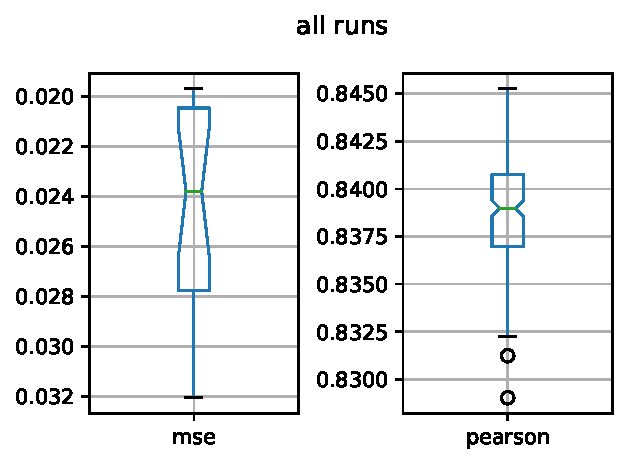
\includegraphics[width=0.9\textwidth]{results/fig_merged.pdf}
%  \caption{Overall model performance as Pearson correlation and MSE.}
%  \label{fig:res_merged}
%\end{figure}

%\begin{figure}[htb!]
%  \centering
%  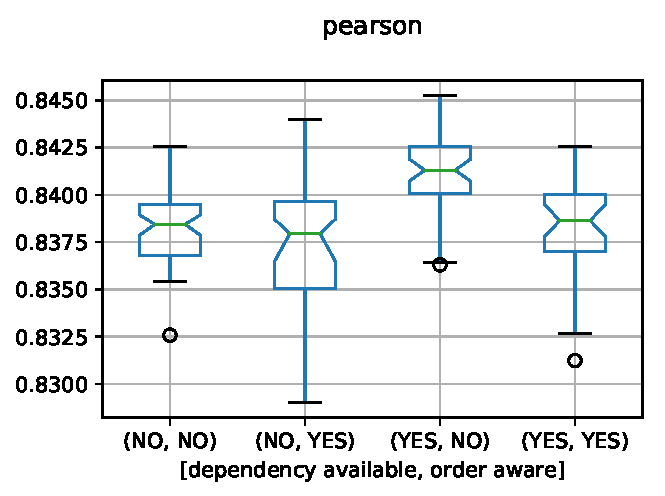
\includegraphics[width=0.9\textwidth]{results/fig_sep_pearson.pdf}
%  \caption{Pearson correlation scores for the different settings.}
%  \label{fig:res_sep_pearson}
%\end{figure}

%\begin{subtable}[c]{\textwidth}
%	\centering
\begin{table}[htb!]
  	\centering
  	%\begin{tabular}{|l|l|l|}
 \begin{tabularx}{
 		\textwidth}{|p{0.26\textwidth} p{0.25\textwidth}|X|X|}%{|X X|X|X|}
 %\begin{tabularx}{\textwidth}{|p{0.21\textwidth} p{0.15\textwidth}|X|X|} %{p{0.4\textwidth}|p{0.4\textwidth}|c}
		\hline
		\texttt{dependency available} & \texttt{order aware} & mse & pearson \\ \hline \hline
		NO & NO & 0.0284 & 0.8382 \\ 
		NO & YES & 0.0206 & 0.8375 \\
		YES & NO & 0.0274 & 0.8413 \\
		YES & YES & 0.0205 & 0.8383 \\ \hline \hline
		\multicolumn{2}{|l|}{TFIDF} & 0.0823 & 0.6189 \\ \hline
 \end{tabularx}
 %\captionsetup{width=0.9\linewidth}
 \caption{MSE and Pearson scores aggregated by setting.}
 \label{tab:results}
\end{table}
%	\vspace*{0.8 cm} \newline
	
  %\caption{Average \ac{MSE} and Pearson's r scores}
%\end{table}


\begin{figure}[htb!]
  \centering
  \textbf{Overall performance by setting}\par\medskip
  \begin{subfigure}{.5\textwidth}
    \centering
    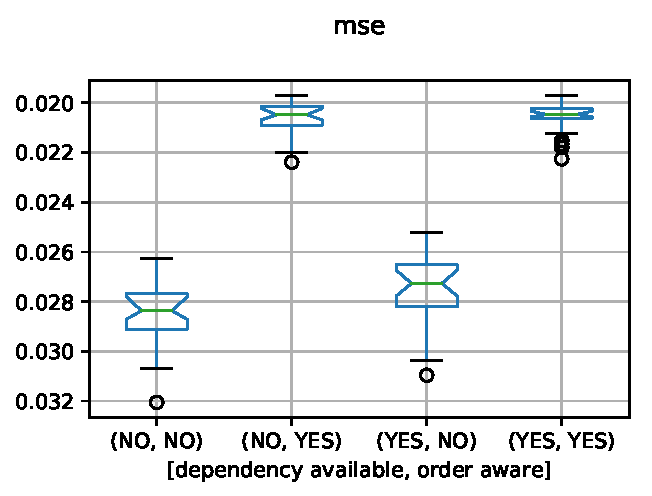
\includegraphics[width=1.\linewidth]{results/fig_sep_mse.pdf}
    \captionsetup{width=0.9\linewidth}
    %\caption{MSE for the different settings (inverted y-axis).}
  \end{subfigure}%
  \begin{subfigure}{.5\textwidth}
    \centering
    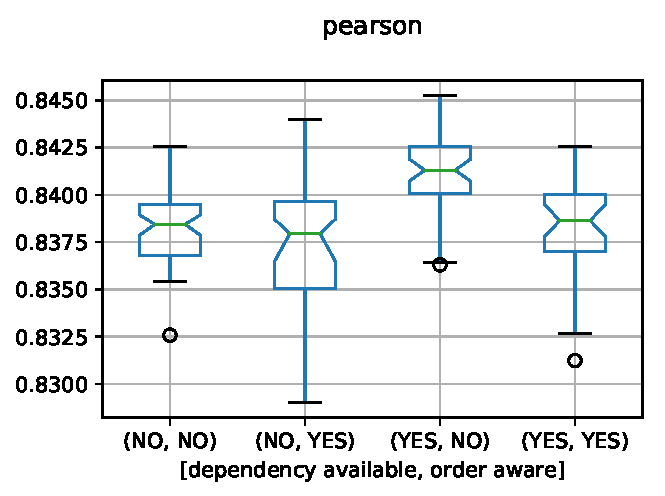
\includegraphics[width=1.\linewidth]{results/fig_sep_pearson.pdf}
    \captionsetup{width=0.9\linewidth}
    %\caption{Pearson's r for the different settings.}
  \end{subfigure}
  \caption{MSE (inverted y-axis) and Pearson's r for the different settings.}
  \label{fig:res_all}
\end{figure}

Adding \textbf{dependency types} improves on average \ac{MSE} by $0.05\%$ and Pearson's r increases by $0.24$ pph, whereby the former is not significant (p=0.336), but the later is ($p<0.0001$). Enabling the feature \textbf{order aware} results in a significant overall performance gain of $0.75$ pph  in means of \ac{MSE} and a performance decrease of $-0.21$ pph with regard to Pearson's r ($p<0.0001$ for two-tailed t-test in both cases). Table~\ref{tab:results_merged} shows the specific scores.

\begin{table}[htb!]
	\centering
	\begin{tabularx}{\textwidth}{|p{0.22\textwidth} p{0.13\textwidth}|p{0.11\textwidth} X|p{0.11\textwidth} X|} 
		%\begin{tabularx}{\textwidth}{|p{0.21\textwidth} X|X|X|} %{p{0.4\textwidth}|p{0.4\textwidth}|c}
		\hline
		parameter & enabled & mse & & pearson  & \\ \hline \hline
		dependency type & NO & 0.0245 & & 0.8378 & \\
		dependency type & YES & 0.0240 & $+0.05$ pph* & 0.8398 & $+0.24$ pph \\ \hline
		order aware & NO & 0.0279 &  & 0.8397 &  \\
		order aware & YES & 0.0206 & $+0.75$ pph & 0.8379 & $-0.21$ pph \\ \hline	   		
	\end{tabularx}
	%\captionsetup{width=0.9\linewidth}
	\caption{Scores aggregated by individual parameter assignment and improvement when enabling the feature. The improvement marked with (*) is not significant.}
	\label{tab:results_merged}
\end{table}

For further study these results that seem to contradict with respect to the applied measure, we took a closer look at the deviations of the predicted relatedness scores from the gold scores. Figure~\ref{fig:fig_sorted_errors_sep} shows the deviations per setting ordered by gold score. It suggests that the averaging model (\texttt{order aware} = NO) overestimates the relatedness score. Indeed, the bias for all predictions in the averaging case ($+8.5$ pph) is significantly ($p < 0.0001$) higher when compared with non-averaging ($+1.9$ pph). Because such a bias distorts the Pearson's~r, and \ac{MSE} was used as cost function while training, we focus at the \ac{MSE} measure for the rest of this work.

\begin{figure}[htb!]
	\centering
	\textbf{Deviations from gold score}\par\medskip
	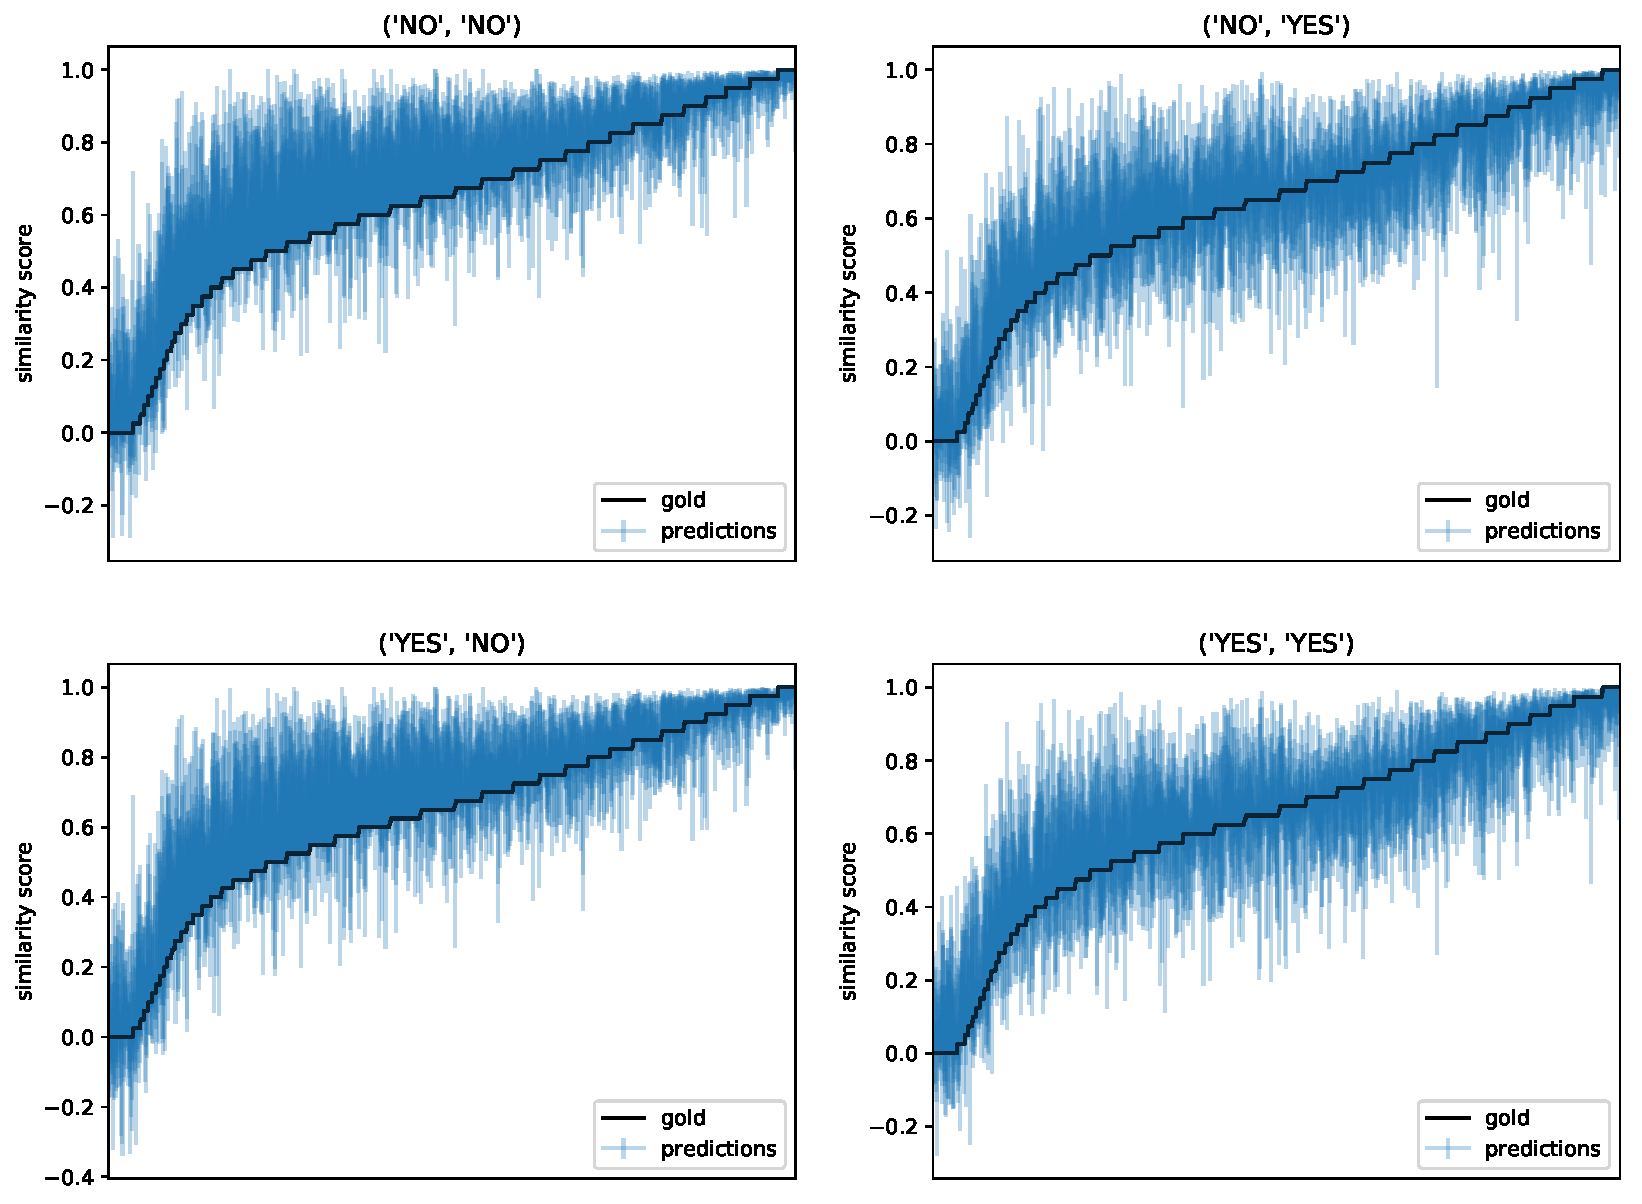
\includegraphics[width=1.\linewidth]{results/fig_sorted_errors_sep.pdf}
	\caption{Deviations of the predictions from gold similarity scores by setting (<\texttt{dependency available}>, <\texttt{order aware}>). The averaging models (\texttt{order aware} = NO; plots at the left) clearly overestimate.}
	\label{fig:fig_sorted_errors_sep}
\end{figure}

\subsubsection{Relation of Order Awareness and Dependency Types} \label{subsec:results_relation_OA_DA}
The specific performance in the examined settings suggests that the parameters \texttt{dependency available} and \texttt{order aware} are related. Figure~\ref{fig:fig_sep_cond} illustrates this by presenting the conditional impact of the parameters. The impact of \texttt{dependency available} seems to vary depending on activation of parameter \texttt{order aware}, whereas the opposite does not hold (see Table~\ref{tab:results} for the actual values). This observation leads to the following question: What kind of useful information with respect to semantical awareness is encoded in dependency types? Precisely, we assume: Dependency types encode local context information that is useful to produce semantic aware compositional representations. The rationale is as follows. 
Order Awareness as implemented within \ac{LSTM}s enable locally contextualized processing (see Section~\ref{subsec:order_aware_composition}). Thus, these models encode local context.
As explained in section \ref{subsec:eval_semantic_awareness}, semantic awareness can be measured using the relatedness prediction task. Since enabling the parameter \texttt{order aware} significantly increases the prediction performance by $+0.8$ pph ($p < 0.0001$) the local context information seems to be important to determine the meaning of a word in a specific textual utterance and to handle semantic aware composition.
Enabling the parameter \texttt{dependency available} significantly improves the model performance by $+0.1$ pph ($p < 0.001$) in the case of disabled order awareness, proving that dependency types indeed encode \textbf{useful} information.
Since the order aware model does not perform significantly better with dependency type data ($t = 0.50$) it seems that this data does not encode extra useful information for order aware models.
This suggests that dependency types indeed encode \textbf{local context}.

\begin{figure}[htb!]
	\centering
	\textbf{Conditional parameter impact}\par\medskip
	\begin{subfigure}{.5\textwidth}
		\centering
		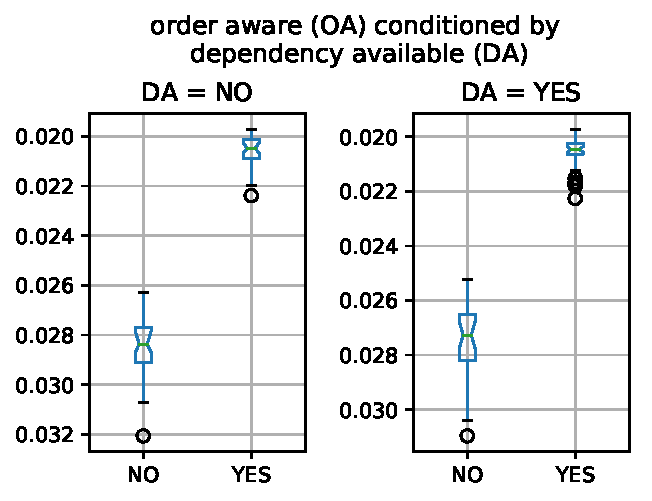
\includegraphics[width=1.\linewidth]{results/fig_sep_cond_order.pdf}
		%\captionsetup{width=0.9\linewidth}
		%\caption{Impact of parameter \textit{order aware} conditioned by enabled \textit{dependency available} parameter.}
	\end{subfigure}%
	\begin{subfigure}{.5\textwidth}
		\centering
		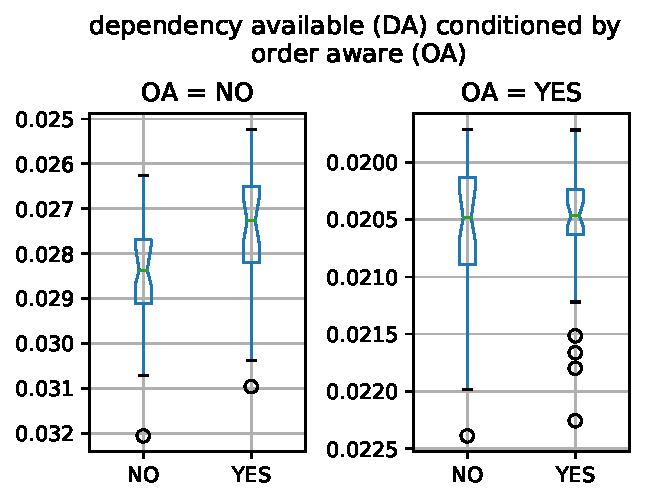
\includegraphics[width=1.\linewidth]{results/fig_sep_cond_dependency.pdf}
		%\captionsetup{width=0.9\linewidth}
		%\caption{Impact of parameter \textit{order aware} conditioned by disabled \textit{dependency available} parameter.}
		\captionsetup{width=0.9\linewidth}
		%\caption{Impact of parameter \textit{dependency available} conditioned by parameter \textit{dependency available}.}
	\end{subfigure}	
	\caption{Conditional parameter impact measured with MSE.}
	\label{fig:fig_sep_cond}
\end{figure}


%\begin{figure}[htb!]
%  \centering
%  \includegraphics[width=0.9\textwidth]{fig_sep_order.pdf}
%  \caption{Influence of order awareness measured with Pearson correlation and MSE.}
%  \label{fig:pearson_all_sep}
%\end{figure}

%\subsubsection{cosine vs. manhattan}
%\subsubsection{Dependency edge types}
%mean mse: 0.0245 -> 0.0240 =  -0.0005 \\
%mean pearson: 0.8378 -> 0.8398 =   0.0019 \\
%performance gain of 0,05\%*/0,31\% (mse/pearson) regarding TF-IDF baseline 

%*: not significant
%\begin{figure}[htb!]
%  \centering
%  \includegraphics[width=0.9\textwidth]{fig_sep_dep.pdf}
%  \caption{Influence of dependency edge type Information measured with Pearson correlation and MSE.}
%  \label{fig:pearson_all_sep}
%\end{figure}



%\subsubsection{Pretraining}

\subsubsection{Value of Dependency Types}
In order to further investigate the value of dependency type data for semantic aware composition we have taken a closer look at the sentence pairs in which only adding this data outperforms the setting in which parameter \texttt{order aware} is enabled exclusively. Table~\ref{tab:results_benefit_DA} lists the top 10 of these data points. Trying to examine the reasons behind cases of superior performance reveals two main classes of constructions (see column \textit{remarks} of Table~\ref{tab:results_benefit_DA}). First, half of the top 10 sentence pairs contains passive constructions. Second, three sentence pairs are related to negation. 

As it turns out, dependency type data seems to be beneficial to handle composition of tokens involved in passive constructions. We filtered the test data set for dependency types indicating these constructions (\textit{auxpass}: passive auxiliary; \textit{nsubjpass}: passive nominal subject; \textit{csubjpass}: passive clausal subject) and calculated \ac{MSE} scores\footnote{We used the relatedness scores predicted by the best model for each setting with respect to train/test split and run.}. Table~\ref{tab:mse_passive} presents the resulting scores and subset sizes. Figure~\ref{fig:fig_mse_passive} visualizes the results. The Dependency Available setting ([YES, NO]) significantly ($p < 0.0001$) outperforms the Order Aware setting ([NO, YES]) in the presence of passive constructions. Furthermore, negation seems to be hard in general. Similar to the passive check, we selected a subset of the test dataset, but filtered by dependency type \textit{neg} and words like "no" or "nobody". For all four settings, the performance dropped significantly when switching from the subset without negation to the negation subset. Despite initial thoughts, negation favors Order Awareness (e.g., performance drop of $-0.2$ pph for [NO, YES] vs. $-0.5$ pph for [YES, NO]) as visualized in Figure~\ref{fig:fig_mse_negation}. Again, Table~\ref{tab:mse_passive} displays the specific evaluation scores and, in addition, relative performance differences with respect to the considered data split.

% pearson-correlation("('NO', 'NO') vs ('YES', 'NO') abs"; "score_jaccard") = -0.456
% > increasing overlap -> decreasing benefit of "dependency available" 
Obviously, the benefit of dependency types decreases with increasing word overlap. Correlating the absolute differences of prediction errors of settings [NO, NO] and [YES, NO] with the Jaccard similarity $f_{S_\text{Jacc}}$\footnote{$f_{S_\text{Jacc}}(s_1, s_2) := \frac{\text{\#(set of tokens in $s_1$ \texttt{AND} $s_2$)}}{\text{\#(set of tokens in $s_1$ \texttt{OR} $s_2$)}}$} of the respective sentences results in a Pearson's r of $-0.46$ indicating a moderate negative correlation.

\begin{table}[htb!]
	\centering
	\begin{tabularx}{\textwidth}{p{0.35\textwidth}|p{0.35\textwidth}|X|X} 
		%\begin{tabularx}{\textwidth}{|p{0.21\textwidth} X|X|X|} %{p{0.4\textwidth}|p{0.4\textwidth}|c}
		\hline
		sentence A & sentence B & errors & remarks \\ \hline \hline
		The patient is being helped by the doctor & The doctor is helping the patient & $-.0;-.5$ (1.0) & passive \\ \hline
		The panda bear is not lying on the logs & A cute panda is lying down & $-.2;-.7$ (0.8) & negation \\ \hline
		A man and a woman are sitting comfortably on the bench & Two large persons are sitting on a park bench and they have a bottle of soda between them & $-.1;-.5$ (0.7) & appended "noise" \\ \hline
		A man is not playing a guitar & A man is playing a keyboard & $-.1;-.4$ (0.7) & negation \\ \hline
		A dog is standing with its two front paws on a rock in a field & A rock is being climbed by the black dog & $-.1;-.4$ (0.6) & passive \\ \hline
		Four middle eastern children, three girls and one boy, are climbing on the grotto with a pink interior & The grotto with a pink interior is being climbed by four middle eastern children, three girls and one boy & $-.0;-.3$ (1.0) & passive \\ \hline
		The flute is being played by one man & A man is playing the guitar loudly & $-.0;-.3$ (0.6) & passive \\ \hline
		Nobody is dangling from straps and kicking at each other & A blonde girl is hanging by gymnastic ropes & $-.1;-.4$ (0.4) & negation \\ \hline
		A child is making a snow ball & A snow ball is being made by a child & $-.0;-.3$ (1.0) & passive \\ \hline
		A black cat and a small white and black cat are looking up at a kitchen countertop & A large dog and a small dog are standing next to the kitchen counter and are investigating & $-.0;-.3$ (0.4) &  \\
		\hline \hline	
	\end{tabularx}
	%\captionsetup{width=0.9\linewidth}
	\caption{The top 10 sentence pairs where enabling \texttt{dependency available} (setting: [YES, NO]) outperforms enabling \texttt{order aware} (setting: [NO, YES]). Rounded deviations from gold scores for both settings ([YES, NO]; [NO, YES]) are presented as \textit{errors} with the actual gold score (rounded) in brackets. The \textit{remarks} column names sources of potentially beneficial effects in favor of the Dependency Available setting.}
	\label{tab:results_benefit_DA}
\end{table}


\begin{table}[htb!]
	\centering
	\begin{tabularx}{\textwidth}{p{0.15\textwidth}|XX|XX|XX|XX|p{0.07\textwidth}} 
		 test data & \multicolumn{2}{c}{[NO, NO]} & \multicolumn{2}{|c|}{[NO, YES]} & \multicolumn{2}{c}{[YES, NO]} & \multicolumn{2}{|c|}{[YES, YES]} & count \\ \hline
		 all & 0.028 & & 0.020 & & 0.026 & & 0.020 & & 4927 \\ \hline
		 w/o passive & 0.028 & & 0.019 & & 0.027 & & 0.020 & & 4371 \\
		 w/ passive & 0.023 & $+0.5\%$ & 0.022 & $-0.3\%$ & 0.021 & $+0.6\%$ & 0.021 & $-0.1\%$ & 556 \\ \hline
		 w/o negation & 0.026 & & 0.019 & & 0.025 & & 0.019 & & 3856 \\
		 w/ negation & 0.032 & $-0.6\%$ & 0.021 & $-0.2\%$ & 0.030 & $-0.5\%$ & 0.021 & $-0.2\%$ & 1071 \\
	\end{tabularx}
	%\captionsetup{width=0.9\linewidth}
	\caption{\ac{MSE} for selected subsets of SICK test data measured within all settings ([<\texttt{dependency available}>, <\texttt{order aware}>]) and relative performance gains/drops (+/-) in pph (\%). \textit{count} represents the number of sentence pairs in the respective subset.}
	\label{tab:mse_passive}
\end{table}

\begin{figure}[htb!]
	\centering
	%\textbf{MSE for specific test data subsets}\par\medskip
	%\caption{MSE for specific test data subsets}
	\textbf{Impact of Order Awareness and Dependency Information \\ in the presence of Passive and Negation}\par\medskip
	\begin{subfigure}[t]{.5\textwidth}
		%\centering
		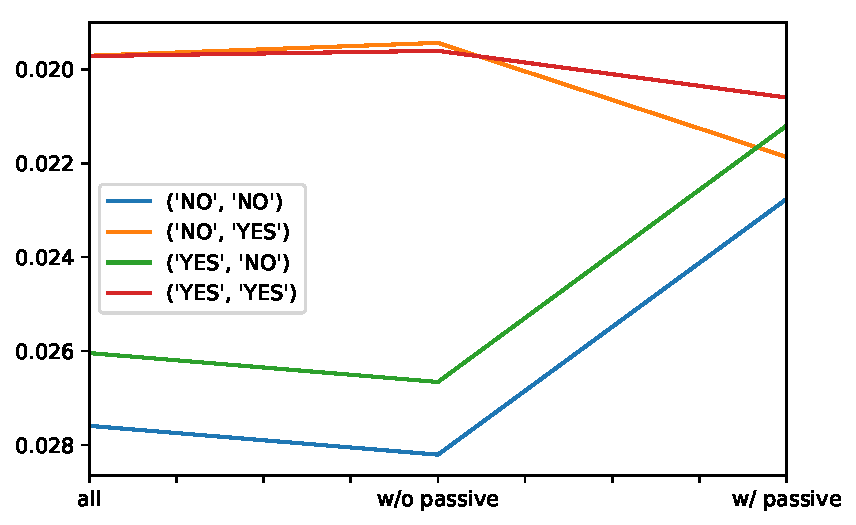
\includegraphics[width=1.\linewidth]{results/fig_mse_passive.pdf}
		\captionsetup{width=0.9\linewidth}
		\caption{The Dependency Available setting ([YES, NO]) outperforms the Order Aware setting ([NO, YES]) on passive constructions.}
		\label{fig:fig_mse_passive}
	\end{subfigure}%
	\begin{subfigure}[t]{.5\textwidth}
		%\centering
		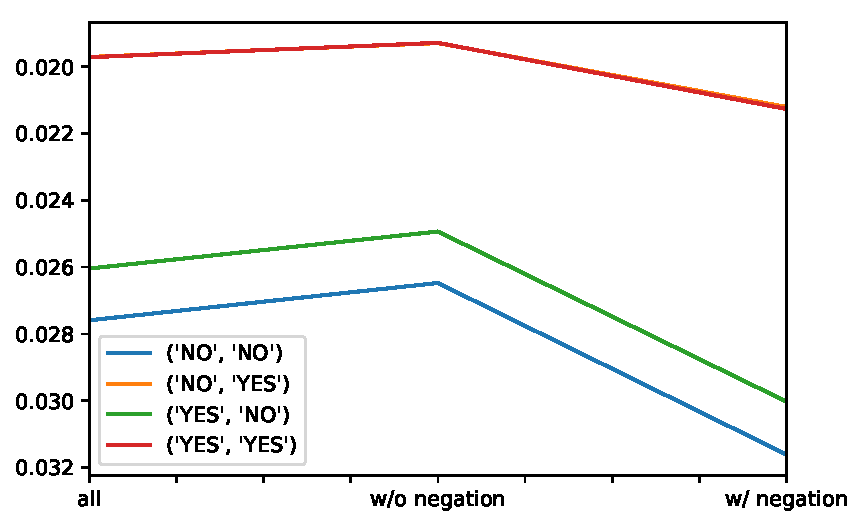
\includegraphics[width=1.\linewidth]{results/fig_mse_negation.pdf}
		\captionsetup{width=0.9\linewidth}
		\caption{The performance decreases for all settings in the presence of negation, but favors Order Awareness ([NO, YES] and [YES, YES]).}
		\label{fig:fig_mse_negation}
	\end{subfigure}	
	\caption{MSE for specific test data subsets}
	%\caption{Conditional parameter impact measured with MSE.}
	%\label{fig:fig_sep_cond}
\end{figure}


\fi
